\chapter{1998:Peter W. Shor}
\label{chap:shor}
\begin{center}
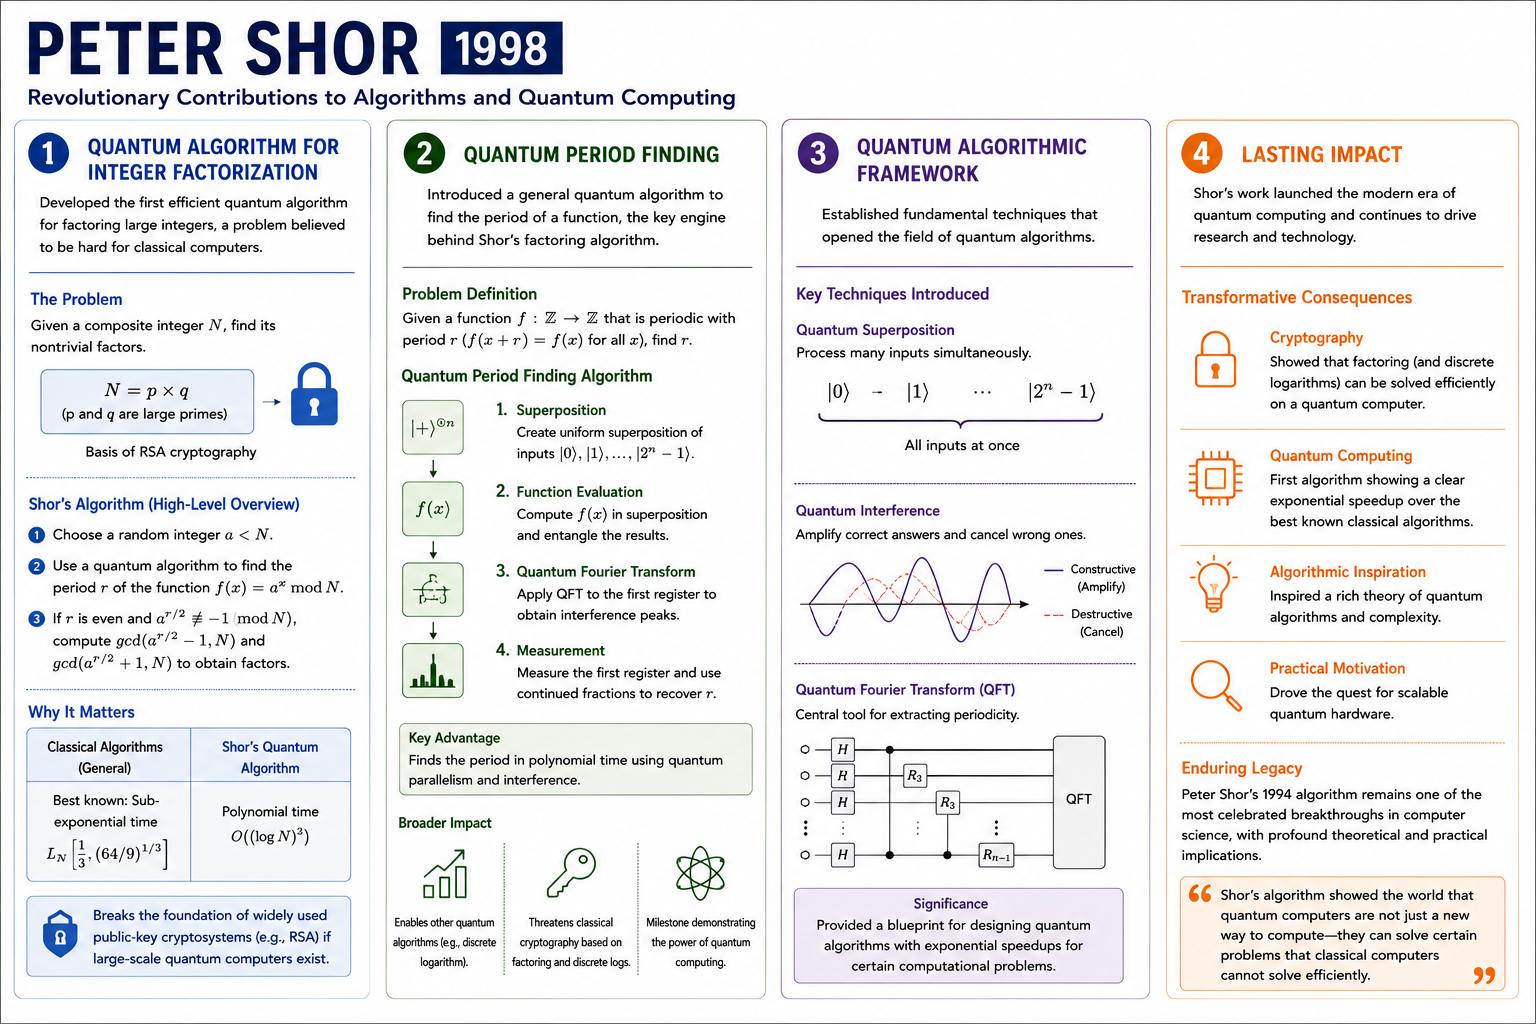
\includegraphics[width=\textwidth]{infographics/abacus5.png}
\end{center}
\targetchapterspacing
\index{Shor, Peter W.}
\booknote{The central habit in this chapter is to hunt for a hidden period, and to ask how interference can make a repeating pattern measurable when sampling one value at a time is too slow.}

\section{An Opening Story: The Wheel and the Strobe Light}

A black wheel with one red dot spins at an unknown rate. Flash a strobe once per second: at the wrong rate the dot darts to a different spot each flash; in time with the wheel it appears frozen. One sample per flash, yet the period is known exactly.

The same trick works when a process repeats every $r$ steps and you may sample it once per step: taken one at a time, the samples look arbitrary. The strobe combines many at once, so combinations agreeing with the true period \emph{add up} and everything else blurs away. Reinforce the compatible, cancel the incompatible---that is the whole mechanism.

In 1998 Peter W. Shor received the Rolf Nevanlinna Prize for building a computer from exactly this mechanism: factoring hides a repeating pattern, and a quantum computer makes it visible and, with the period, obtains the factors.

\section{The Problem}

\noindent\textbf{Factoring.} Multiplying is fast: $23\times 41=943$; reversing it is not. Trial division works for small numbers, but for an $n$-bit $N$, trying all primes up to $\sqrt{N}$ costs about $2^{n/2}$ steps---astronomical at $n=200$. The best classical methods (Pollard's rho, the quadratic sieve, the number field sieve) are still not polynomial: for an $n$-bit input, the number field sieve needs roughly $\exp\!\bigl(c\,n^{1/3}(\log n)^{2/3}\bigr)$ steps. Nobody has proved factoring hard; the belief rests on fifty years of failed attempts.

\noindent\textbf{Why it matters.} Public-key cryptography lives on this asymmetry. In RSA the public key is a product $N=pq$; anyone can encrypt, but only someone knowing $p$ and $q$ can decrypt. The related \emph{discrete logarithm} problem---find $x$ given $g^x\equiv h\pmod p$ for a prime $p$, or the analogous problem on an elliptic curve---protects key exchange and signatures. Both bet that reversing an easy computation is hard.

\noindent\textbf{The physics, in one paragraph.} A qubit is a superposition $\alpha\lvert 0\rangle+\beta\lvert 1\rangle$ with $|\alpha|^2+|\beta|^2=1$; amplitudes can add and cancel, but measuring samples one outcome---0 with probability $|\alpha|^2$---and only that survives. Is there a problem whose difficulty comes from sampling one thing at a time, that a machine built to interfere amplitudes could solve instead?

\section{The World Before}

Factoring grew harder to do as it grew more useful: trial division covers a few digits, Pollard's rho tens of digits, the quadratic sieve reached 100 digits in 1991, and the number field sieve passed 250 digits in the 2020s. All remain subexponential, and RSA keys grew from 512 bits to 2048 because the multiply-versus-factor gap seemed safe.

Quantum computing had a quieter history. Feynman (1982) suggested a quantum machine might be the only efficient way to \emph{simulate} quantum physics; Deutsch (1985) and Deutsch--Jozsa (1992) separated quantum from classical machines only on problems with no practical use. As of the early 1990s no quantum algorithm beat the best classical one on any realistic task, and many doubted a useful quantum algorithm existed.

The doubt was grounded: $n$ qubits represent $2^n$ inputs at once, but measure and you get one random outcome with all structure discarded. \emph{Parallelism alone is not power.} Missing was a way to process amplitudes \emph{before} measuring---letting them add and cancel so a meaningful statistic survives.

\section{The New Idea}

\subsection{Factoring becomes a hidden period}

The pivot is classical number theory: \emph{factoring reduces to finding a period.} Choose $a$ sharing no factor with $N$ (say $a=7$, $N=15$). The powers $a^1,a^2,a^3,\ldots$ modulo $N$ take finitely many values, so they repeat; since $a$ and $N$ share no factor, the first repeated value is $a^1$ itself. The sequence cycles with period $r$, the least positive integer with $a^r\equiv 1\pmod N$, called the \emph{order} of $a$ modulo $N$. Computing powers until the pattern returns---the classical way to find $r$---is the slow, sample-by-sample search the strobe defeats.

What makes $r$ valuable: if $r$ is even and $a^{r/2}\not\equiv -1\pmod N$, then
\[
\gcd(a^{r/2}-1,\,N)\quad\text{and}\quad\gcd(a^{r/2}+1,\,N)
\]
are genuine factors of $N$. Indeed $N$ divides $(a^{r/2}-1)(a^{r/2}+1)$ because it divides $a^r-1$, yet neither factor alone---otherwise the order would be smaller, or $a^{r/2}\equiv-1$---so each gcd pulls out a proper divisor. Finding the factors \emph{is} finding the period.

\subsection{Quantum period-finding: interference does the searching}

Before Shor, a computation was a step-by-step pipeline from input to output. The new idea: compute $a^x\bmod N$ for many $x$ in superposition, then apply an operation that converts \emph{periodic} input into \emph{concentrated} output---the quantum Fourier transform (QFT). A classical Fourier transform already has the strobe's property: a signal of period $r$ concentrates its energy in a few frequencies; a random signal spreads it. The quantum version does this to amplitudes, which can interfere: outcomes agreeing with the hidden period reinforce, others cancel. A measurement then lands, with high probability, on a frequency carrying the period; continued fractions recover $r$, and the number theory above turns it into factors. The speedup is not ``trying every answer at once'': interference moves probability toward answers agreeing with the period and silences the rest.

\subsection{Quantum error correction: protecting the fragile}

A long computation faces a second enemy: the state decays. Classical error correction copies bits and compares---but quantum states cannot be copied, and measuring a qubit collapses it. Shor's solution spreads one \emph{logical} qubit across several \emph{physical} ones and measures carefully chosen combinations whose values reveal which error occurred without revealing the information itself. Redundancy plus a syndrome, arranged so checking does not disturb what it protects. Below a physical error threshold, arbitrarily long computations become possible in principle.

\section{How It Works: Worked Examples}

\subsection{Factoring 15 by order-finding}

Factor $N=15$ by finding the order of $a=7$. First, $\gcd(7,15)=1$. Compute powers modulo 15:
\begin{align*}
7^1&=7,\\
7^2&=49\equiv 4\pmod{15} &&(49-45=4),\\
7^3&=4\cdot 7=28\equiv 13\pmod{15} &&(28-15=13),\\
7^4&=13\cdot 7=91\equiv 1\pmod{15} &&(91-90=1).
\end{align*}
The first power equal to 1 is the fourth, so the order is $r=4$.

Since $r=4$ is even, $a^{r/2}=7^2=49\equiv 4\pmod{15}$, and $4\not\equiv 14\equiv-1\pmod{15}$, so the formula applies:
\[
\gcd(7^2-1,\,15)=\gcd(48,15)=3,\qquad
\gcd(7^2+1,\,15)=\gcd(50,15)=5.
\]
The factors appear directly: $15=3\cdot 5$.

The quantum part supplies $r=4$ without the four-step search: its output is a frequency, and continued fractions recover the denominator 4. The algorithm is probabilistic in two ways: the order may be odd, or $a^{r/2}$ may be $-1$---then the formula fails and one retries with a different $a$; and the measured frequency only approximates a fraction with denominator $r$, so a few runs suffice. The final arithmetic is exact; only the search is probabilistic.

\subsection{A strobe in frequency space: the Fourier transform of a repeating pattern}

Take the length-four signal $[1,0,1,0]$, period 2. Its discrete Fourier transform is $X_k=x_0+x_1\omega^k+x_2\omega^{2k}+x_3\omega^{3k}$, where $\omega=e^{-2\pi i/4}$ is a quarter-turn, so $\omega^2=-1$ and $\omega^4=1$:
\begin{align*}
X_0&=1+0+1+0=2,\\
X_1&=1+1\cdot\omega^2=1-1=0,\\
X_2&=1+1\cdot\omega^4=1+1=2,\\
X_3&=1+1\cdot\omega^6=1-1=0.
\end{align*}
The transform is $(2,0,2,0)$: two peaks, two exact zeros. Repetition has become concentration, exactly as the strobe freezes a wheel; all the mass sits at frequency 0, the constant part, and frequency 2, the rate of repetition.

Contrast the non-repeating signal $[1,1,1,0]$: its transform is $X_0=3$, $X_1=-i$, $X_2=1$, $X_3=i$, magnitudes $(3,1,1,1)$---energy spread across every frequency. In the periodic case the entries agreeing with the repetition add up and the others cancel to zero. The quantum Fourier transform performs this interference on amplitudes, so a single measurement sees the peak and not the noise.

\section{The Mathematics in Brief}

A qubit is a unit vector $\alpha\lvert 0\rangle+\beta\lvert 1\rangle$ with $|\alpha|^2+|\beta|^2=1$; measuring samples 0 or 1 with those probabilities and collapses the state. Several qubits carry $2^n$ coefficients, but an algorithm may touch them only through unitary operations and measurements.

\noindent\textbf{Order.} For $\gcd(a,N)=1$, the \emph{order} $r$ is the least positive integer with $a^r\equiv 1\pmod N$; the sequence $a^x\bmod N$ repeats with period $r$.

\noindent\textbf{The factor-recovery identity.} If $r$ is even and $a^{r/2}\not\equiv -1\pmod N$, then $\gcd(a^{r/2}-1,N)$ and $\gcd(a^{r/2}+1,N)$ are nontrivial factors of $N$. \emph{Why it is true:} $N$ divides $(a^{r/2}-1)(a^{r/2}+1)$ yet divides neither factor, so each gcd lies strictly between 1 and $N$.

\noindent\textbf{The quantum Fourier transform.} A signal of period $r$ has a Fourier transform concentrated at frequencies whose denominators divide $r$. \emph{Why it is true:} values spaced $r$ apart carry identical phase and add; the others spread around the circle and cancel. Shor's algorithm superposes $a^x\bmod N$, applies the QFT, and measures; continued fractions recover $r$ from the measured frequency.

\noindent\textbf{Error correction.} One logical qubit is encoded across many physical qubits, and syndrome measurements reveal errors without revealing the logical state. The threshold theorem: below a physical error rate determined by the code and noise model, arbitrarily long computations become reliable with modest overhead; above it, adding qubits can make things worse.

\noindent\textbf{Where the speed comes from.} The gain is interference, not parallelism: the machine never reads every answer; it arranges amplitudes so answers compatible with the hidden period keep their probability and incompatible answers lose it, then measures once.

\section{Limits and Modern Views}

Current devices remain noisy and far below the fault-tolerant scale required for a cryptographically relevant factorization; the exact physical-qubit count depends on the platform and changes rapidly. Resource estimates commonly place such a computation in the millions of physical qubits. The threshold theorem is a statement about a noise model, not a guarantee about any chip; correlated errors and imperfect operations can violate its assumptions. The theorem, the resource estimate, and the engineering forecast are three different claims; the theory establishes the first, while the third remains open \cite{shor-factoring,shor-error}.

What is threatened, precisely? Systems whose security rests on factoring or discrete logarithms, such as RSA and conventional Diffie--Hellman or elliptic-curve key exchange. Symmetric cryptography (AES, SHA) is different: the best generic quantum attack, Grover's search, only squares the effective security, so doubling the key length restores it. Post-quantum cryptography seeks replacements believed hard even for quantum machines---lattices, error-correcting codes, and hash-based constructions are leading families; isogeny-based proposals remain a research direction after major candidate failures. None is unconditionally safe; each is a bet on an assumption.

\section{Exercises and Self-Study Guide}
\begin{enumerate}[label=\textbf{E\arabic*.}]
\item Verify the factor-recovery formula on another pair: take $N=21$, $a=2$. Compute the powers of 2 modulo 21, find the order, and use the gcd identity to factor 21.
\hint{Follow the 15 example line by line. The order is 6, $2^3=8\not\equiv -1\pmod{21}$, and the two gcds are 7 and 3.}
\item Compute the powers of $a=14$ modulo 15, find its order, and apply the gcd identity. Explain why this $a$ is a poor choice for the algorithm.
\hint{The order is 2 and $a^{r/2}=14\equiv-1\pmod{15}$; the two gcds come out 1 and 15, not proper factors.}
\item Explain why measuring a qubit destroys access to its amplitudes. Give the state $\alpha\lvert 0\rangle+\beta\lvert 1\rangle$ and describe what happens to $\alpha$ and $\beta$ after one measurement.
\hint{After the measurement the state is $\lvert 0\rangle$ or $\lvert 1\rangle$; one amplitude has vanished. Write the probabilities of the two outcomes before the collapse.}
\item Explain why superposition alone is useless, using the coin metaphor: $n$ qubits represent $2^n$ values, yet a measurement returns one random outcome.
\hint{Unless amplitudes were engineered beforehand, the chance that a single sample hits a useful answer is exponentially small.}
\item Compute the discrete Fourier transform of the length-eight signal $[1,0,1,0,1,0,1,0]$ and state where its peaks sit.
\hint{All nonzero entries lie at even positions, so each $X_k$ is a sum of four unit vectors spaced a quarter-turn apart; they add to 4 only at $k=0$ and $k=4$.}
\item List every assumption hidden in a threshold-theorem statement, and identify which one an engineer could measure on a real device.
\hint{Errors are assumed independent or local; gates and measurements must be accurate enough; correction must run fast enough. The effective per-operation error rate is what to measure.}
\item Separate cryptographic primitives into those threatened by order-finding and those affected only by generic quantum search. Justify each placement.
\hint{Order-finding attacks anything built on modular exponentiation, such as RSA and discrete-logarithm key exchange; Grover's search only halves the effective key length of a hash or block cipher.}
\end{enumerate}

\booknote{A final exercise in judgment: before celebrating any quantum speedup, ask what structure the interference is amplifying. If you cannot name the hidden period---the pattern the amplitudes are agreeing on---then the advantage, like the strobe's frozen wheel, may be an illusion of coherence rather than a real discovery.}
\clearpage
